\chapter{Background}


\section{Skein Theory}

\subsection{Foundations and General Notions}
In this work, we will be forced to discuss a few different variants of skein modules. For this reason, it will be useful to first describe some general framework of skein theory so that each of these variants will be a special case. Unless otherwise stated, we will assume $M$ is an oriented $3$-manifold with boundary $\partial M$ (possibly empty), $\Sigma$ is an oriented surface, $I$ is the real interval $[0,1]$, $R$ is a commutative and unital ring. 

\begin{definition}
    Let $T_1, T_2: X \to M$ be smooth embeddings of a smooth manifold $X$ into $M$. A \textbf{smooth ambient isotopy} $H: T_1 \Rightarrow T_2$ is a smooth homotopy of diffeomorphisms $H_t: M \to M$ such that $H_0=\id_M$ and $H_1 \circ T_1 = T_2$. Furthermore, we demand that the boundary $\partial M$ is fixed by the homotopy. 
\end{definition}

The relation 
\[
T_1 \sim T_2 \textrm{ if and only if there exists a smooth ambient isotopy } H: T_1 \Rightarrow T_2
\]
is an equivalence relation. The smoothness requirement of $H$ is important when considering knots. Without it, all knots would be equivalent to the unknot by contracting all of the complexity of the knot to a point. 

\begin{definition}
Let $N$ be a finite set of points contained in the boundary $\partial M$. An \textbf{$N$-tangle} in $M$ (or just \textit{tangle} for short) is the smooth ambient isotopy class of a smooth embedding 
\[
T: \underbrace{\underset{j \in J}{\bigsqcup}\, S^1}_{:=L} \sqcup \underbrace{\underset{k \in K}{\bigsqcup}\, I}_{:=B} \to M
\]
for some finite sets $J$ and $K$ such that
\begin{enumerate}
\item the image of $L$ lies in the interior of $M$,
\item the image of the interior of $B$ lies in the interior of $M$,
\item the image of the boundary of $B$ equals $N$.
\end{enumerate}
If $B$ is empty, then the result is called a \textbf{link} in $M$. Similarly, if $L$ is empty, then it's called a \textbf{braid} in $M$. 

One may also consider \textit{oriented} or \textit{framed} tangles by choosing an orientation or framing for each point in $N$ and for each connected component of $L$ and $B$ such that the choices are compatible with each other with respect to the smooth embedding.
%For our purposes, the difference between framed and unframed tangles will be a matter of convention; we choose to work with framed tangles as is standard in the literature. 
If $M = \Sigma \times I$, then we will assume that the points in $N$ are contained in $\Sigma \times \{ \frac{1}{2} \}$ and that their framings are thought to be embedded orthogonally to $\Sigma \times \{ \ast \}$. 
\end{definition}

We say a framed tangle in $\Sigma \times I$ has \textbf{blackboard framing} if the entire framing is embedded orthogonally to $\Sigma$. Every framed link in $\Sigma \times I$ is isotopic to one with a blackboard framing by turning each twist into a loop with a local blackboard framing:

\[
    \vcenter{\hbox{\includegraphics[height=3cm]{twist.eps}}} \quad = \quad \vcenter{\hbox{\includegraphics[height=3cm]{invvh2.eps}}}.
\]
This suggests that we may represent framed links in $\Sigma \times I$ as link diagrams on $\Sigma$. Indeed, equivalence under ambient isotopy is captured by the Reidemeister moves 2, 3, and a modified Reidemeister move 1:

\[
    \vcenter{\hbox{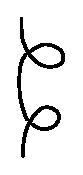
\includegraphics[height=3cm]{modifiedr1.eps}}} \quad = \quad \vcenter{\hbox{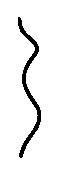
\includegraphics[height=3cm]{modifiedr1resolution.eps}}}.
\]

\AP{Add pictures of RII and RIII for good measure.}
Below are some examples of framed tangle diagrams.

\[
    \vcenter{\hbox{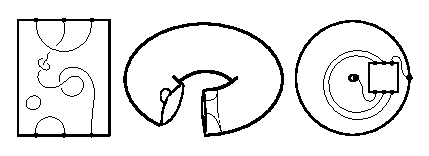
\includegraphics[height=3cm]{Ntangles.eps}}}
\]
\AP{fix torus picture by removing band.}

Define the \textbf{writhe} of a tangle diagram is the number of positive crossings minus the number of negative crossings. It is easy to see that the Reidemeister moves above preserve the writhe of a diagram, so the concept is well defined. Writhe should be thought of as a grading on the free $R$-module on the set of tangles in the given space, which provides a good reason to work with framed links over ordinary links. Such a module is a main ingredient of this theory, so let's honor it with a proper discussion.

\begin{definition}
Let $\ct(M, N)$ be the free $R$-module generated by the set of framed $N$-tangles in $M$. Analagously, we can define $\ct^{or}(M,N)$ to be the free $R$-module generated by the set of oriented framed $N$-tangles in $M$. All definitions which are to follow in this subsection have an analagous definition using oriented tangles. Also, we will formally define $\cs_R(\varnothing, \varnothing) := R$. 
\end{definition}

The construction $\ct( -, -)$ is actually a symmetric monoidal functor $\ct: \sfc \to R\textsf{-Mod}$ for a careful choice of category $\sfc$ which we now describe. The objects of $\sfc$ are pairs $(M, N)$ of the same type as discussed previously. A morphism $(f, W): (M', N') \to (M, N)$ is a pair of a smooth, orientation-preserving embedding $f: M' \to M$ such that $M - f(M')$ is either a smooth 3-manifold or the empty set, and choice of $W \in \ct\big( M-f(M'), N \sqcup f(N') \big)$ (unless $M - f(M')$ is empty, in which case $W$ is a formal symbol for the "empty link" in the empty set). Composition is given by $(g, W') \circ (f, W) = (g \circ f, W' \cup W)$, which is associative since $\circ$ and $\cup$ are associative.

\AP{Give a picture of composition in $\sfc$.}

The induced map denoted $W: \ct(M', N') \to \ct(M, N)$ is a linear map defined by $W(T) = W \cup T$, and we will refer to such a linear map $W$ as a \textbf{wiring}. We are abusing notation by denoting this linear map by $W$, but it should be clear from the context what $f$ is since it is technically encoded in the data of the element $W \in \ct\big( M-f(M'), N \sqcup f(N') \big)$. It is true that $\ct$ preserves composition and identity morphisms, making and so $\ct$ is functorial. $\sfc$ can now be equipped with a symmetric monoidal structure via disjoint union. It is clear that 
\[\ct_R(M \sqcup M', N \sqcup N') \cong \ct_R(M, N) \underset{R}{\otimes} \ct_R(M', N')\]
for any sets of framed points $N \subset \partial M$ and $N' \subset \partial M'$. The unit is given by the object $(\varnothing, \varnothing) \in \sfc$ and define $\ct(\varnothing, \varnothing) := R$, which makes $\ct$ a symmetric monoidal functor. 

\begin{definition}
Let $B$ be the smooth closed $3$-ball, $N_i$ be a choice of $2i$ boundary points of $B$, and let $X \subset \underset{i \in \N}{\bigsqcup} \ct(B, N_i)$ be some (typically finite) set, which we will call a set of \textbf{skein relations}. Given any tangle module $\ct(M, N_M)$, there exists a submodule $\ci(X)$ generated by the set 
\[\{ W(x) \mid x \in X \text{ and } W:\ct(B, N_B) \to \ct(M, N_M) \text{ is a wiring diagram} \}.\] 
A quotient of the form $\cs_X(M, N) := \ct(M, N) / \ci(X)$ is called a \textbf{skein module} of $M$ relative to $N$. If $N = \varnothing$ is the empty set, we may use the notation $\cs_X(M) := \cs_X(M, \varnothing)$. Similar definitions may be given using oriented and/or unframed tangles instead. 
\end{definition}
The construction $\cs_X(-, -)$ is a functor in the same way that $\ct(-, -)$ is; a smooth, orientation-preserving embedding $f: M \to M'$ and an element $W \in \cs_X\big( M-f(M'), N \sqcup f(N') \big)$ (assume $N$ is disjoint from $\im(f)$) defines a linear map $W: \cs_X(M, N) \to \cs_X(M', N')$. In fact, the quotient maps $\alpha_{(M, N)}: \ct(M, N) \to \cs_X(M, N)$ yield a natural transformation. In other words, given a morphism $(M, N) \to (M', N')$ in $\sfc$, the diagram
\begin{center}
\begin{tikzcd}
	\ct(M, N) \arrow[d,"\alpha_{(M, N)}"] \arrow[r, "W"] 
	& \ct(M', N') \arrow[d, "\alpha_{(M', N')}"]\\
	\cs_X(M, N) \arrow[r, "W"] & \cs_X(M', N')
\end{tikzcd}
\end{center}
commutes. Such a functor will be called a $\textbf{skein theory}$ (or \textit{oriented} skein theory if the skein relations are based on oriented tangles). 

For any oriented surface $\Sigma$, we can define a category $\sfskein_X(\Sigma)$ which we will call a $\textbf{skein category}$. The objects of this category are finite sets of framed points (together with a choice of orientation if the skein theory is oriented) $N$ in $\Sigma$, and the morphisms $N \to N'$ are elements of $\cs_X\big(\Sigma \times I, (N \times \{0\}) \sqcup (N' \times \{1\})\big)$, so the category is $R$-linear. Write composition of morphisms by concatenation. If $y:N \to N'$ and $z:N' \to N''$ are morphisms, then their composite $yz:N \to N''$ is constucted by gluing $z$ on $y$ through $N'$ and rescaling the interval coordinate appropriately.

\AP{Picture of composition in $\sfskein_X(\Sigma)$.}

The endomorphism algebras in this category are called \textbf{skein algebras} and are denoted by $\cs_X(\Sigma, N) := \cs_X(\Sigma \times I, (N \times \{0\}) \sqcup (N \times \{1\}) \big)$. If $N$ is the empty set, then we reduce the notation to simply $\cs_X(\Sigma)$.

If $f: \Sigma \to \Sigma'$ is a smooth embedding of surfaces, then there is an induced functor 
\[
\sfskein_X(f): \sfskein_X(\Sigma') \to \sfskein_X(\Sigma)
\]
defined on objects by $\sfskein_X(f)(N) = f(N)$ and on morphisms in the following way. First, extend $f$ trivially to $f \times \id_I: \Sigma \times I \to \Sigma' \times I$. Then, in the skein algebra of the complement of the image of $f \times \id_I$, choose the multiplicative identity element $e \in \cs_X\big( \Sigma' - \im(f) \big)$ which is the empty tangle. The pair $(f \times \id_I, e)$ is an object in the category $\sfc$, which gives rise to a wiring
\[e: \cs_X\Big(\Sigma \times I, \big(N \times \{0\}\big) \sqcup \big(N' \times \{1\}\big) \Big) \to \cs_X\Big(\Sigma' \times I, \big(f(N) \times \{0\}\big) \sqcup \big( f(N') \times \{1\} \big) \Big)\]
via the functor $\cs_X$. Now we may define what $\sfskein_X(f)$ does to morphisms: $\sfskein_X(f)(y) = e(y)$ for any $y \in \cs_X\Big(\Sigma \times I, (N \times \{0\}) \sqcup (N' \times \{1\}) \Big)$.

\AP{Picture of how $\sfskein_X(f)$ works on morphisms.}

It is clear that $\sfskein_X(f)$ preserves composition and identity morphisms. Therefore, if we let $\mathsf{Surf}$ be the category of smooth embeddings between smooth oriented surfaces, we can summarize our last few points by saying we have a functor
\[
\sfskein_X: \mathsf{Surf} \to \mathsf{Cat}.
\]
In particular, $\sfskein_X(f)$ defines algebra homomorphisms on the skein algebras
\[e: \cs_X\big(\Sigma, N\big) \to \cs_X\big(\Sigma', f(N)\big).\]
\AP{We use this type of algebra homomorphism when we embed the annulus into the torus.}

\begin{remark} \label{rem:skeinaction}
The above homomorphisms are a special case of a more general type of map. If $N$ is a set of framed points on $\Sigma$, then a smooth embedding $f: \Sigma \to \partial M$ induces a $\cs_X(\Sigma, N)$-module structure on $\cs_X\big(M, N'\big)$ for any $N'$ with $f(N) \subseteq N'$. The action is given by ``pushing tangles in through the boundary". In other words, the pre-composition of a smooth embedding of a collar neighborhood $g: \partial M \times I \to M$ with $f \times \id_I: \Sigma\times I \to \partial M \times I$ induces a bilinear map
\[
\cs_X(\Sigma, N) \times \cs_X(M, N') \to \cs_X(M, N')
\]
because $M$ minus a collar neighborhood is diffeomorphic to itself. Alternatively, a choice of element in $\cs_X(\Sigma, N')$ produces a wiring $\cs_X(M, N') \to \cs_X(M, N')$.

\AP{Picture of action.}
\end{remark}


\subsection{Examples of Skein Theories}

The last subsection leaves us with an important and unanswered question. Which sets of skein relations $X$ produce interesting skein theories? One class of examples is found by importing sets of relations satisfied by morphisms in a linear ribbon category as skein relations. Ribbon categories are braided monoidal categories which are rigid and equipped with a twist morphism for every object, satisfying some compatibility conditions. The axioms are such that the morphisms may be interpreted as framed braid diagrams. In particular, the morphisms satisfy the Reidemeister moves shown previously. We will discuss three examples of skein theories derived from skein relations which are meant to emulate linear relations satisfied by the braid and twist morphisms in certain ribbon categories coming from the representation theory of quantum groups, a topic which has generated a lot of interest from mathematicians since the 1980s. The categories of representations of quantum groups are ribbon categories with non-involutive braidings and the skein relations below capture how far off the braidings are from being involutive.  

Here, we are forced to fix a base ring. For our purposes, $R$ must be a commutative ring containing invertible elements $s$ and $v$. Typical choices of $R$ are $\Z[s^{\pm 1}, v^{\pm 1}], \Q(s, v)$, or some other ring in between these.  In particular, the theorem \AP{Cite BB} is stated over this ring, a result we will depend heavily on later on. \\

\begin{example}[\textit{Kauffman (Dubrovnik) Skein Relations}]
Let $X'$ be the set of two unoriented skein relations
\begin{flalign*}
    (1) \quad \vcenter{\hbox{\includegraphics{poscross.eps}}} &= \vcenter{\hbox{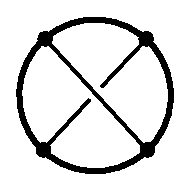
\includegraphics{negcross.eps}}} + (s-s^{-1}) \,\, \vcenter{\hbox{\includegraphics{idresolution.eps}}} - (s-s^{-1}) \,\, \vcenter{\hbox{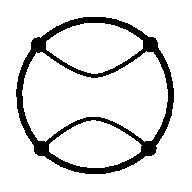
\includegraphics{capcupresolution.eps}}} \\ \\
    (2) \quad \vcenter{\hbox{\includegraphics{vh.eps}}} &= v \,\, \vcenter{\hbox{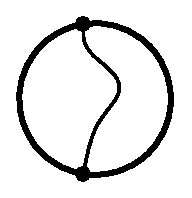
\includegraphics{frameresolution.eps}}}.
\end{flalign*}
The functor $\cd(-,-) := \cs_{X'}(-,-)$ is the Dubrovnik skein theory (sometimes just called the Kauffman skein theory). We will use the notation $\mathsf{D}(-) := \sfskein_{X'}(-)$ for the Dubrovnik skein categories. Using the Dubrovnik variant is important for us (see \AP{universal enveloping algebra result}). This theory is related to Dubrovnik polynomials in that the Dubrovnik polynomial of a link is a normalized value of the link in $\cd(S^3)$. The normalization is often so that the Dubrovnik polynomial of the unknot is $1$, whereas the value of the unknot in $\cd(S^3)$ is $\delta_\cd := 1 - \frac{v-v^{-1}}{s-s^{-1}}$, which can be deduced from the skein relations.
\end{example}

\begin{example}[\textit{HOMFLYPT Skein Relations}]
Next, let $X''$ be the set of two oriented skein relations
\begin{flalign*}
    (1) \quad \vcenter{\hbox{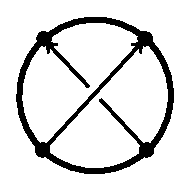
\includegraphics{poscrossor.eps}}} &= \vcenter{\hbox{\includegraphics{negcrossor.eps}}} + (s-s^{-1}) \,\, \vcenter{\hbox{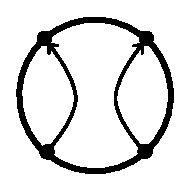
\includegraphics{idresolutionor.eps}}} \\ \\
    (2) \quad \vcenter{\hbox{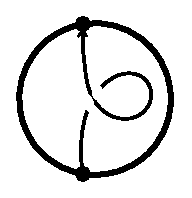
\includegraphics{vhor.eps}}} &= v \,\, \vcenter{\hbox{\includegraphics{frameresolutionor.eps}}}.
\end{flalign*}
The functor $\ch(-,-) := \cs_{X''}(-,-)$ is the HOMFLYPT skein theory and we use the notation $\mathsf{H}(-) := \sfskein_{X''}(-)$ for the HOMFLYPT skein categories. As in the Dubrovnik case, this theory is related to HOMFLYPT polynomials so that the HOMFLYPT polynomial of a link is a normalized value of the link in $\ch(S^3)$. Again, some often make the choice to normalize this polynomial so that the value of the unknot is $1$, but the value of the unknot in $\ch(S^3)$ is $\delta_\ch := -\frac{v-v^{-1}}{s-s^{-1}}$.
\end{example}

\begin{example}[\textit{Kauffman Bracket Skein Relations}]
As a final example, let $X'''$ be the set of two unoriented skein relations
\begin{flalign*}
    (1) \quad \vcenter{\hbox{\includegraphics{poscross.eps}}} &= s \,\, \vcenter{\hbox{\includegraphics{idresolution.eps}}} + s^{-1} \,\, \vcenter{\hbox{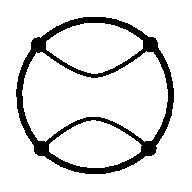
\includegraphics{capcupresolution.eps}}} \\ \\
    (2) \quad \vcenter{\hbox{\includegraphics{vh.eps}}} &= -s^{-3} \,\, \vcenter{\hbox{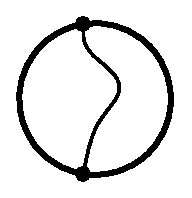
\includegraphics{frameresolution.eps}}}.
\end{flalign*}
The functor $\ck(-,-) := \cs_{X'''}(-,-)$ is the Kauffman bracket skein theory (not be confused with the Kauffman skein theory) and we use $\mathsf{K}(-) := \sfskein_{X'''}(-)$ to notate the Kauffman bracket skein categories. The value of a link in $\ck(S^3)$ is equal to its bracket polynomial, which may be normalized as above to obtain its Jones polynomial. 
\end{example}

\begin{remark}
Any linear combination of tangles which satisfy the Dubrovnik skein relations will also satisfy the Kauffman bracket skein relations after making the specialization $v=-s^{-3}$. Therefore, there is a natural transformation of skein theories $\eta: \cd(-,-) \to \ck(-,-)$ induced by the intentity map on link diagrams. 
\end{remark}

In this work, we will be focused on generalizing existing results from the HOMFLYPT and Kauffman bracket skein theories to the Dubrovnik skein theory, but we will state a few facts regarding the HOMFLYPT and Kauffman bracket skein theories when it is valuable for us to do so. 

\AP{Maybe add a remark about Turaev's work on deformations of the Goldman Lie algebras? Could potentially say a lot to motivate the topic, but I'm not super familiar with a lot of it.}

\subsection{Skein algebras of tangles in a cube}

In the case where $\Sigma = I \times I$, the endomorphism objects of $\mathsf{D}(\Sigma), \mathsf{H}(\Sigma)$, and $\mathsf{K}(\Sigma)$ are known and provide the motivation for why the choices of skein relations are what they are. For an integer $n \geq 1$, let $[n]$ be a set of $n$ points in $\Sigma$, chosen to be evenly spaced along the line segment $\{ 1/2 \} \times I$ (choose all points share the same orientation in the context of an oriented skein theory). Then the endomorphism algebras 
\[
BMW_n := \End_\mathsf{D}(\Sigma)([n]), \qquad H_n := \End_\mathsf{H}(\Sigma)([n]), \qquad TL_n := \End_\mathsf{K}(\Sigma)([n])
\]
are known to be isomorphic to the Birman-Murakami-Wenzl, (Type A) Hecke, and Temperley-Lieb algebras, respectively (\AP{*Add citations}). 

Let $q \in \C$ be not a root of unity, $U_q(\mathfrak{gl}_N)$ be the Drinfeld-Jimbo quantum group associated to the Lie algebra $\mathfrak{gl}_N$, and $V$ be the natural representation of $U_q(\mathfrak{gl}_N)$ (\AP{cite Chari-Pressley book}). Then $H_n$ acts on the $n$-fold tensor product $V^{\otimes n}$ by $U_q(\mathfrak{gl}_N)$-linear endomorphisms, and this action generates $\End_{U_q(\mathfrak{gl}_N)}(V^{\otimes n})$. This is actually part of the statement of quantum Frobenius-Schur-Weyl duality: $V^{\otimes n}$ is a $U_q(\mathfrak{gl}_N)$-$H_n$-bimodule, and the action of one algebra generates the linear endomorphisms with respect to the other. So a representation of one algebra determines a representation of the other via tensor product with $V^{\otimes n}$. The Birman-Murakami-Wenzl algebra plays the role of the Hecke algebra for $U_q(\mathfrak{g}_N)$ in the case where $\mathfrak{g}$ is one of the orthogonal or symplectic Lie algebras. For this reason, from a Lie theoretic point of view, the HOMFLYPT skein theory is thought of as a ``type A" theory, while the Dubrovnik skein theory is a ``types B, C, D" skein theory.

As for the Temperley-Lieb algebra $TL_n$, it acts on the $n$-fold tensor power $V^{\otimes n}$ of the natural representation of $U_q(\mathfrak{gl}_2)$. Actually, there is a surjective algebra homomorphism $\pi_{TL}: H_n \to TL_n$ and the action $H_n \to \End_{U_q(\mathfrak{gl}_2)}(V^{\otimes n})$ factors through this homomorphism (see \AP{cite Jimbo}). One can conclude that the action of $H_n$ on $V^{\otimes n}$ is not faithful, at least in the case when $N=2$ and $n \geq 2$. \AP{sl2 vs gl2?}

Much is known about these algebras and some of the results surrounding them are very useful in our context. One of the main ideas is that each of the algebras discussed above has a family of idempotents which provide algebraically nice closures to links in the skein algebra of an annulus. Let's first describe the Hecke algebra in more detail before focusing on the BMW algebra. 

For any partition $\lambda$ of $n$, there exists an element $y_\lambda \in H_n$ which is idempotent, so that $y_\lambda^2 = y_\lambda$, and minimal in the sense that it generates a minimal left-ideal of $H_n$ (see \AP{cite Aiston-Morton}). The elements $y_n := y_{(n)}$ corresponding to single row partitions are called \textbf{(Hecke) symmetrizers}. These elements have a certain absorption property which makes them unique, which we will now describe. Let us use $\sigma_i \in H_n$ be the positive crossing between the $i^{\rm{th}}$ and $(i+1)^{\rm{th}}$ strands. 
\AP{Picture of oriented $\sigma_i \in H_n$.}
The algebra $H_n$ is generated by the $\sigma_i$ and the symmetrizers are the unique idempotent elements satisfying $\sigma_i y_n = s y_n = y_n \sigma_i$. In this way, $y_n$ corresponds to a $1$-dimensional representation of $H_n$ (it is a deformation of the trivial representation of $\C S_n$ where $s=1$).

A similar story holds for the BMW algebra. Firstly, $BMW_n$ is generated by positive crossing elements $\sigma_i$ and cap-cup elements $c_i$. 
\AP{pictures of $\sigma_i$ and $c_i$}
The $c_i$ generate a proper ideal $I_n$ in $BMW_n$. In (\AP{cite BB}), the authors show that the complement of $I_n$ in $BMW_n$ is isomorphic to $H_n$, giving an isomorphism $BMW_n \cong H_n \oplus I_n$. Then they construct an additive and multiplicative (but non-unital) homomorphism 
\[
\Gamma_n : H_n \to BMW_n
\]
which is a section of the natural projection $BMW_n \to H_n$ such that 
\begin{equation} \label{eq:bbsectionproperty}
\Gamma_n(x)y = 0 = y \Gamma_n(x) \quad \textrm{for } x \in H_n, y \in I_n.
\end{equation}
Using this section, one can transport the minimal idempotents $y_\lambda \in H_n$ to minimal idempotents $\tilde{y}_\lambda := \Gamma_n(y_\lambda) \in BMW_n$. The elements $\tilde{y}_n := \tilde{y}_{(n)}$ are called the \textbf{(BMW) symmetrizers} and are the unique idempotent elements of $BMW_n$ satisfying the properties of the Hecke symmetrizers and property \eqref{eq:bbsectionproperty}. By \AP{cite Shelly}, these symmetrizers satisfy a very useful recurrence relation
\begin{equation} \label{eq:shellyrecurrence}
*=*
\end{equation}
\AP{Change $f_n$ to $\tilde{y}_n$ in symmetrizer pictures.}
\AP{Define quantum integers and $\beta_n$}
%\[
%[n+1] \vcenter{\hbox{\includegraphics[width=2.9cm]{f_nplus1.eps}}} = [n]s^{-1} \vcenter{\hbox{\includegraphics[width=2.9cm]{f_notimes11otimesf_n.eps}}} + \vcenter{\hbox{\includegraphics[width=2.9cm]{sigma_ndotssigma_11otimesf_n.eps}}} + [n]s^{-1} \beta_n \vcenter{\hbox{\includegraphics[width=2.9cm]{f_notimes1H1otimesf_n.eps}}}.
%\]
For what it's worth, this relation descends to a recurrence relation for the $y_n \in H_n$ via the projection map described above ($\tilde{y}_n$ gets sent to $y_n$ and the last diagram on the right-hand side gets sent to $0$). 

\AP{Come back and add braiding/twist identities from BB if we need them.}

\AP{This next diagram actually doesn't commute... $\pi_H(c_i)=0$, but $\eta_{\dots}(c_i) = c_i$. What does this mean for images of BMW symmetrizers in $TL_n$? Discuss Jones-Wenzl projectors once this is figured out since they are needed for compatibility result.}
\begin{center}
\begin{tikzcd}
	& BMW_n \arrow[dl, "{\pi_H}", two heads] \arrow[dd, "{\eta_{(I^3, 2n)}}", two heads] \\
H_n \arrow[dr, "{\pi_{TL}}", two heads] \arrow[ur, "\Gamma", bend left, hook] & \\
	& TL_n
\end{tikzcd}
\end{center}

\subsection{Skein Algebras of the Annulus}

Let's use the notation $A := S^1 \times [0,1]$ for the annulus. The thickened annulus represents perhaps the simplest space with non-trivial topology that can harbor links. There are often many different smooth embeddings of the thickened annulus into a given 3-manifold $M$ (one for every element of $\pi_1(M)$, at the very least). Keep in mind that if we have a smooth embedding $f: A \times I \hookrightarrow M$, then we have an induced linear map between skein modules $\cs_X(f): \cs_X (A) \to \cs_X (M)$, allowing us to prod for information about $\cs_X(M)$. One useful type of embedding of $A$ is into a tubular neighborhood of a knot, which is often called \textit{decorating} or \textit{threading} a knot.

A first observation is that any skein algebra of the form $\cs_X(A)$ is commutative because the link algebra $\cs_\varnothing(A)$ is a commutative algebra. To see this, consider the product of two links $L_1$ and $L_2$ in the link algebra and start by stretching $L_2$ towards the outer boundary past $L_1$, followed by moving it down below the furthest point of $L_1$, and finally contracting $L_2$ can to its original radial position. 

We'll tackle describing the structure of $\ck(A)$ before the others since it is the easiest. The Kauffman bracket skein relation allows one to resolve all crossings in any diagram on any surface $\Sigma$. It is a theorem of Pzytycki that the set of non-trivial mutli-curves (non-trivial meaning that no curve bounds a disk), together with the empty link in $A \times \{ \ast \}$ forms a basis of $\ck(A)$ (actually, the theorem is stated for any skein algebra, see \AP{cite}). There is only one non-trivial curve $z$ and the set $\{ z^k \}_{k \in \N}$ exhaust all of the multicurves. Therefore, $\ck(A)$ is a polynomial algebra $R[z]$. 

The HOMFLYPT and Dubrovnik cases are more complicated because the skein relations do not allow one to resolve all the crossings in a diagram. However, they do allow one to change a diagram with a negative crossing into a diagram with a positive crossing, plus diagrams with a lesser number of crossings. It follows that the skein algebras $\ch(A)$ and $\cd(A)$ are generated by knots with only positive crossings. Let $z_i$ be a knot in $A$ with winding number $i$ around the annulus. Turaev shows in \AP{cite} that the $z_i$ are algebraically independent by showing their HOMFLYPT and Dubrovnik polynomials are algebraically independent. Therefore, $\ch(A)$ is a polynomial algebra $R[z_i, i \in \Z_{\neq 0}]$. $\cd(A)$ has half as many generators since the $z_i$ in that setting are unoriented, but $\cd(A)$ is a polynomial algebra $R[z_i, i \in \Z_{> 0}]$ by the same arguments. 

\AP{Picture of $z_i$}

The skein algebras of tangles in a cube relate to the skein algebras of the annulus via a map $\cl(-)$, depicted as a wiring diagram below. 

\AP{Picture of closure}

Let $\widetilde{Q}_\lambda := \cl(\tilde{y}_\lambda)$ and use the shorthand notation $\tilde{h}_n := \widetilde{Q}_{(n)}$ for the BMW symmetrizer closures. Zhong and Lu show in \AP{cite} that the set $\{ \widetilde{Q}_\lambda \}_\lambda$ forms a basis of $\cd(A)$ over the base ring $R=\Q(s, v)$, where $\lambda$ ranges over all paritions. Actually, it is an eigenbasis with respect to the meridian map
\AP{picture of meridian map.}
where the eigenvalue of $Q_\lambda$ is 
\[
c_\lambda = \delta_\cd + ( s - s^{-1} ) \sum_{\square \in \lambda} v^{-1} s^{2 \textrm{cn}(\square)} - v s^{-2 \textrm{cn}(\square)}
\]
and where $\textrm{cn}(\square) := j - i$ is the \textit{content} of the box in the $\square$ in $i^\textrm{th}$ row and $j^\textrm{th}$ column of the Ferrer's diagram of the partition $\lambda$. Two distinct partitions $\lambda$ and $\lambda '$ give rise to distinct values of $c_\lambda$ and $c_\lambda'$. Therefore, each of the eigenspaces is $1$-dimensional. 

The behavior of $\widetilde{Q}_\lambda$ is similar to that of the $Q_\lambda := \cl^+(y_\lambda) \in \ch(A)$ where $\cl^+(-)$ is defined by orienting the strands in wiring digram of $\cl(-)$ counter-clockwise, as we now describe. Using the description $\ch(A) = R[z_i, i \in \Z_{\neq 0}]$, consider the subalgebras $\ch(A)^+ := R[z_i, i \in \Z_{> 0}]$ and $\ch(A)^- := R[z_i, i \in \Z_{< 0}]$. Then the two subalgebras are isomorphic via the linear involution defined by $z_i \mapsto z_{-i}$ and $\ch(A) \cong \ch(A)^+ \otimes \ch(A)^-$. The $\{ Q_\lambda \}_\lambda$ forms an eigenbasis of $\ch(A)^+$ with resepect to the meridian map and the eigenspaces are $1$-dimensional. As a side remark, the linear involution $z_i \mapsto z_{-i}$ may be realized topologically by rotating the thickened annulus $\pi$ radians around an appropriately centered axis parallel to $A$ and taking the induced skein map. We will call this map the \textit{flip map}.

In \AP{cite Lukac}, it's shown how to interpret $\ch(A)^+$ as the ring of symmetric functions $\Lambda$ (also see \AP{cite Morton Murphy Operators}). There is an injective algebra homomorphism $\Lambda \to \ch(A)^+$ which sends the complete homogeneous symmetric function $h_n$ to $Q_{n}$ (such a map exists because $\Lambda$ is a free commutative $\Z$-algebra over the set $\{ h_n \}_{n \geq 1}$, see \AP{cite Macdonald}). Under this homomorphism, the Schur function $s_\lambda$ is sent to $Q_\lambda$. This theorem has plenty of implications. For example, the structure constants of $\Lambda$ in the basis $\{ s_\lambda \}_\lambda$ are the Littlewood-Richardson coefficients, which are then sent to structure constants of $\ch(A)^+$ in the basis $\{ Q_\lambda \}_\lambda$. In Chapter \AP{reference}, we discuss partial results surrounding the Dubrovnik analogue of this homomorphism. See Section \AP{reference} for a summary about the ring $\Lambda$.

Another application of the interpretation of $\ch(A)^+$ as $\Lambda$ is the definition of new special links in the skein algebra. There is a family of elements known as the power-sum symmetric functions, whose counterparts in $\ch(A)^+$ we will denote by $P_n$. These elements are algebraically independent in $\Q \otimes \Lambda$. Therefore, monomials in the $P_n$ form a basis of $\ch(A)^+$.


\subsection{Skein Algebras of the Torus}

The power-sum elements $P_n \in \ch(A)$ described above are known to behave wonderfully in skein theoretic computations. This allows for a simple description of the HOMFLYPT skein algebra of the torus $\ch(T^2)$ in terms of generators and relations. First, let's define the generators. For any rational number $r$ there is a smooth embedding 
\[
\iota_{r}: A \to T^2
\]
of the annulus into a tubular neighborhood of the line of rational slope $r$ in the torus. Consider the embeddings $\iota_{r}$ and $\iota_{-r}$ to be the same embedding with opposite orientations. These induce an algebra homomorphisms
\[
\ch(\iota_r): \ch(A) \to \ch(T^2)
\]
on the level of skein algebras. The $\iota_r$ are distinct isotopically (even homotopically) and are exhaustive in the sense that any knot in the thickened torus is may be represented as being contained in the image of an $\iota_q$. Therefore, any basis of $\ch(A)^+$ defines a basis of $\ch(T^2)$. Let's consider this with respect to the the power-sum monomial basis of $\ch(A)^+$. More precisely, for any pair of integers $\xx = (a, b)$ where $k = \gcd(\xx)$, define 
\[
P_\xx := \ch(\iota_{a/b})(P_k).
\]

In \AP{cite MS}, Morton and Samuelson prove that the skein algebra $\ch(T^2)$ admits a presentation with generators the elements of $\{ P_\xx \mid \xx \in \Z^2 \}$, subject to the relations 
\[
[P_\xx, P_\yy] = \big( s^{\det(\xx,\yy)} - s^{-\det(\xx,\yy)} \big) P_{\xx + \yy}.
\]
This presentation exhibits a relationship to the elliptic Hall algebra, a 2-parameter family of algebras obtained via Hall algebra decategorification of categories of coherent sheaves over certain elliptic curves (see \AP{Burban-Schiffman}). Along the diagonal of the parameter space, the Burban-Schiffman presentation of the elliptic Hall algebra matches the Morton-Samuelson presentation of the skein algebra of the torus. At the very least, this highlights two things. Firstly, the skein algebra of the torus admits a known deformation. Secondly, skein algebras are connected to surprising areas of mathematics and hence deserve our attention. \AP{Is this paragraph correct?}

What we describe next is the Kauffman bracket skein algebra of the torus, although the order of exposition is opposite to the historical order of discovery. The story is actually quite similar to the HOMFLYPT case. Recall that $\ck(A)$ is a polynomial algebra $R[z]$ where $z$ is the simple closed curve around the hole of the annulus with winding number $1$. There exist polynomials known as \textit{Chebyshev polynomials} $T_k \in R[z]$ for all integer $k \geq 1$ which form a basis of $\ck(A)$. For any pair of integers $\xx = (a, b) \in \Z^2$, define elements $e_\xx \in \ck(T^2)$ as 
\[
T_\xx := \ck(\iota_{a/b})(T_k).
\]
Note that $e_\xx = e_{-\xx}$ because the $T_k$ are fixed under the flip map, which is possible since the Kauffman bracket skein theory is an unoriented skein theory. With this in mind, we may pass to the smaller indexing set $Z^2 / \langle \xx = -\xx \rangle$. Using these elements, Frohman and Gelca \AP{cite} prove that the skein algebra $\ck(T^2)$ admits a presentation with generators $T_\xx$ subject to the relations
\[
T_\xx T_\yy = s^{\det(\xx, \yy)} T_{\xx + \yy} + s^{-\det(\xx, \yy)} T_{\xx - \yy}
\]
which the authors call the ``product-to-sum" formulas. There is an algebra called the \textit{noncommutative torus}, which is a one-parameter deformation of the algebra of continuous functions on the torus. The Frohman-Gelca presentation of $\ck(T^2)$ matches a presentation of the invariant subalgebra of the noncommutative torus with respect to a certain involutive action, as shown in \AP{cite FG}. \AP{Is this paragraph correct?}

Given the similarity between the presentations of $\ch(T^2)$ and $\ck(T^2)$, one might suspect that there exists a similar description of the Dubrovnik skein algebra $\cd(T^2)$. The answer to this question is affirmative, which is what we discuss in Chapter \AP{How to reference a chapter?}


\subsection{A Relative Skein Algebra of the Annulus}

At this point in the story we have introduced special links in the skein algebras of the annulus and described how we can transport these into other skein modules via threading knots. In order to say anything meaningful about these threadings, we ought to know how these special links will interact with other links once in the resulting space. For example, is there an easy way to describe how can we pass a special link through a single strand of another link? To answer this question universally, we should answer it in a certain relative skein algebra which is the endomorphism algebra of one point in the skein category of the annulus. Appropriate wirings from this skein algebra into other skein modules will give us our desired description. Here we will describe this algebra in more detail and summarize what is already known. 

First we will restrict ourselves to the HOMFLYPT case, for which we summarize the results from \AP{Morton, Murphy operators}. The object we would like to discuss is $\ca_\ch := \ch(A, [1])$, which is depicted diagramatically as an annulus with one point on each boundary component. This algebra is closely related to the affine Hecke algebra of type A, $\dot{H}_1$ (see \AP{cite MS}). Two of the most basic elements of $\ca_\ch$ are
\AP{Pictures of identity $e$ and once around counter-clockwise $a$.}
The product in the algebra in this digrammatic notation is given by nesting annuli. 

Let $\cc_\ch := \ch(A)$. Then, $\cc_\ch$ admits both a left $\cc_\ch$-action by pushing links infront of tangles in $\ca_\ch$.
\AP{Picture of left action.}
It is known that there is an equality of algebras between $\ca_\ch$ and the Laurent polynomial algebra $\cc_\ch[a^{\pm 1}]$. In particular, $\ca_\ch$ is commutative and the left action is determined by how it acts on $e$.  

Analagously, there is a right $\cc_\ch$-action by pulling links in behind tangles in $\ca_\ch$. 
\AP{picture of right action.}
Both actions are examples of those arising from embeddings into the boundary of the thickened annulus, as described in Remark \ref{rem:skeinaction}. The left and right actions obviously commute, endowing $\ca_\ch$ with a $\cc_\ch$-$\cc_\ch$-bimodule structure. It is probably worth pointing out that the left action is not equal to the right action. A simple measurement of how far off the two actions are from being equal would answer our question posed above. The answer is given as a commutator relation 
\begin{equation} \label{eq:pkcommutator}
P_k \cdot e - e \cdot P_k = (s^k - s^{-k}) a^k.
\end{equation}
\AP{Make sure this order is correct.}
The proof involves the definition of a certain wiring diagram, defining a linear map $H_n \to \ca_\ch$. The idempotents $y_{n}$ satisfy a certain recurrence relation, and the commutator relation above follows from writing $P_k$ in terms of the $y_n$ and calculations involving the image of this recurrence relation.

Eventually we would like to prove a Dubrovnik analogue of Equation \eqref{eq:pkcommutator}, but we still haven't defined any Dubrovnik analogue of the $P_k$ (see \AP{ref}). Nevertheless, we can discuss some of what was previously known about the algebra $\ca_\cd := \cd(A, [1])$ (see \AP{Shelly} for more details). 

Let $\cc_\cd := \cd(A)$ and let $a, e \in \ca_\cd$ be the unoriented versions of the elements of the same name above. As in the HOMFLYPT case, there is a left-$\cc_\cd$ action on $\ca_\cd$ and the algebra $\ca_\cd$ is equal to the Laurent polynomial algebra $\cc_\cd[a^{\pm 1}]$. There is also a right-$\cc_\cd$ action on $\ca_\cd$, endowing $\ca_\cd$ with a bimodule structure. 

Consider the wiring diagrams
\AP{pictures of wirings. I would drop the subscript on $W_n$ for brevity and rename $\widetilde{W}$ to $W^*$ to not confuse with $\tilde{y}_n$.}
which define linear maps $BMW_n \to \ca_\cd$. Let $W_n := W(\tilde{y}_{n+1})$ and $W^*_n :=  W^*(\tilde{y}_{n+1})$ where the subscript denotes the ``winding number'' around $A$. Taking the image of Equation \eqref{eq:shellyrecurrence} under $W$ gives a relation
\begin{equation} \label{eq:recursionina1}
[n+1] W_n = e \cdot \tilde{h}_n + [n] s^{-1} a W_{n-1} + [n] s^{-1} \beta_n a^{-1} W^*_{n-1}.
\end{equation}

There are maps
\[
	(-)^*: BMW_n \to BMW_n \qquad \overline{(-)}: BMW_n \to BMW_n
\]
induced by the diffeomorphisms of the thickened square $(x, y, t) \mapsto (x, 1-y, 1-t)$ and $(x, y, t) \mapsto (x, y, 1-t)$, respectively. The map $\overline{(-)}$ is often called the \emph{mirror map} and is an $R$-anti-linear involution, while $(-)^*$ will be called the \emph{flip map} and is an $R$-linear involution. The symmetrizers $\tilde{y}_n$ are fixed under these maps because the mirror and flip maps preserve the properties which make $\tilde{y}_n$ unique.
Using the quotient map defined by the equivalence relation $(x, 0, t) \sim (x, 1, t)$, we may analagously define maps
\[
	(-)^*: \ca_\cd \to \ca_\cd, \qquad \overline{(-)}: \ca_\cd \to \ca_\cd
\]
which are linear and anti-linear involutions, respectively. We will also call these the flip map and the mirror map; it will be clear from the context which is being applied. These maps satisfy the relations
\begin{align*}
	\left( W \left( x \right) \right)^* &= W^* \left( x^* \right), & (y \cdot e)^* &= e \cdot y^*, \\
	\overline{W \left( x \right)} &= W \left( \overline{x} \right), & \overline{(y \cdot e)} &= e \cdot \overline{y}
\end{align*}
for any $x \in BMW_n$ or $y \in \cc_\cd$. Apply the flip, the mirror, and the composite of the two separately to Equation \eqref{eq:recursionina1} to obtain alternate versions of the original recurrence relation:
\begin{equation} \label{eq:recursionina2}
\quad [n+1] W^*_n = \tilde{h}_n \cdot e + [n] s^{-1} a W^*_{n-1} + [n] s^{-1} \beta_n a W_{n-1}, 
\end{equation}
\begin{equation} \label{eq:recursionina3}
[n+1] W_n = \tilde{h}_n \cdot e + [n] s a W_{n-1} + [n] s \bar{\beta}_n a^{-1} W^*_{n-1},
\end{equation}
\begin{equation} \label{eq:recursionina4}
\quad [n+1] W^*_n = e \cdot \tilde{h}_n + [n] s a^{-1} W^*_{n-1} + [n] s^{-1} \bar{\beta}_n a W_{n-1}.
\end{equation}

Rearranging the difference of Equations \eqref{eq:recursionina1} and \eqref{eq:recursionina2} gives a relation
\begin{equation}
\tilde{h}_n \cdot e - e \cdot \tilde{h}_n = \{n\} (a^{-1} W^*_{n-1} - a W_{n-1})
\end{equation}
which Shelly calls a \textit{fundamental skein relation} in $\ca_\cd$ since it reduces to to usual Dubrovnik skein relation when $n=1$. \AP{This might also be true in another sense, since there might be some connection between the $W_n$ and something called the ``tube algebra", as pointed out by Henry Tucker.} In Chapter \AP{??}, we will provide a similar relation which amounts to rewriting the right-hand side of the equation in terms of elements of the form $h_i \cdot a^k$ (alternatively $a^k \cdot h_i$). 

\section{The Ring of Symmetric Functions}

\subsection{Character Rings of Classical Groups}

\subsection{Bases of $\Lambda$ and Identities}